\chapter{Imaging}\label{c:imaging}

\section{Detector Cuts}

Approximately xxx \% of the detectors in the array can not be used to generate images.
For some the detector membranes are broken.
Others appear intact upon visual inspection, but show no response to applied current even in the superconducting state.
Others work as expected while superconducting, but can not be biased so as to show a response to changes in optical power. 
And some are extremely noisy or consistently show other problems in the data stream.
This section summarizes which detectors have each of these problems.
\figref{fig:detector-cuts-wafer} and \figref{fig:detector-cuts-rc} contain plots summarizing this information graphically, organized by detector position on the wafer and by readout row/column respectively..

To determine which detectors show no response in the superconducting state, the temperature of the focal plane was set to 975~mK, well below the $T_c$ of the detectors.
The \TES\ bias current was ramped, and data was acquired while running the readout system open-loop.
\figref{fig:tes-bias-ramp-sc} shows the resulting data for rows 0 -- 4 of all columns.
Most row/column combinations show a response that maps out the $V$-$\Phi$ curve for the SQUID amplifier chain.
The row/column combinations that show no response indicate either a broken detector line, a broken SQUID on a mux chip, broken wirebonds, or some other problem in the readout system.

Another group of detectors remain superconducting at the chosen bias point and operating temperature of 1100~mK.
This could be caused by an abnormally high $G$ value, or by a short somewhere in the \TES\ circuit.
\figref{fig:tes-bias-ramp-trans} shows the result of ramping \TES\ bias current while running the readout system open-loop, but while the system is at 1100~mK and the \TESs\ are biased into the transition at a DAC value of 27000.

\begin{figure*}[th]
\centering
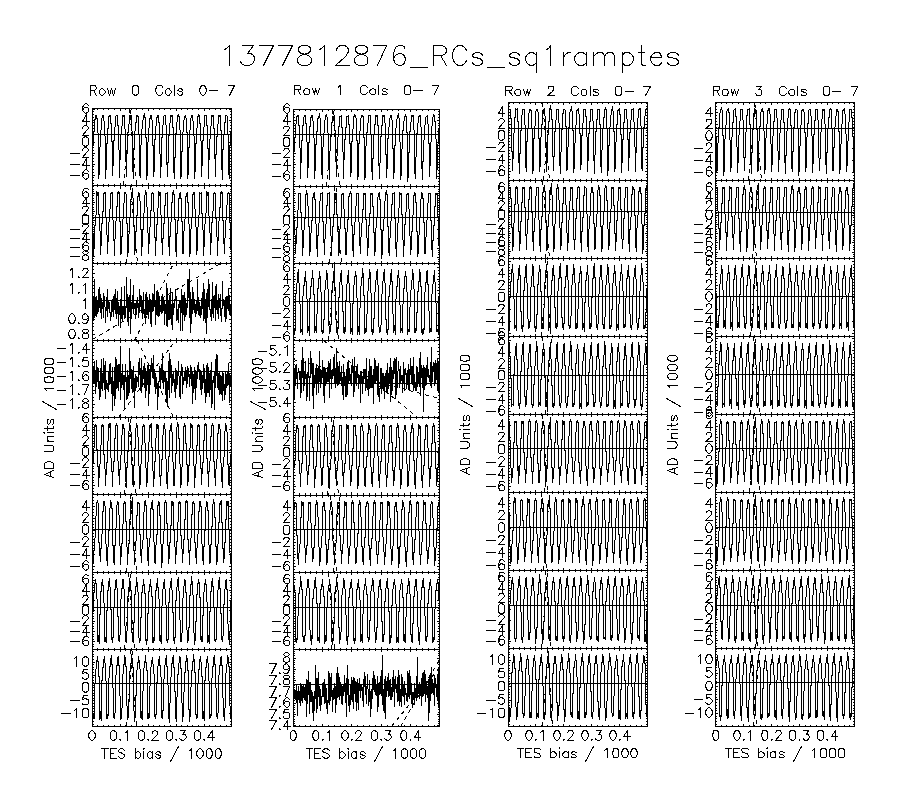
\includegraphics[width=\textwidth]{\here/../images/1377812876_RCs_sq1ramptes_00.png}
\caption{Plot showing response of SQUID amplifier chain to ramp in \TES\ bias current, while \TES\ is superconducting.. Data is shown for rows 0--4 for all eight columns. \RC{0}{2}, \RC{0}{3}, \RC{1}{3}, \RC{1}{7} all show no response, only noise (note the change in vertical scale for these row/columns). xxx need to explain units on axes?}
\label{fig:tes-bias-ramp-sc}
\end{figure*}

\begin{figure*}[th]
\centering
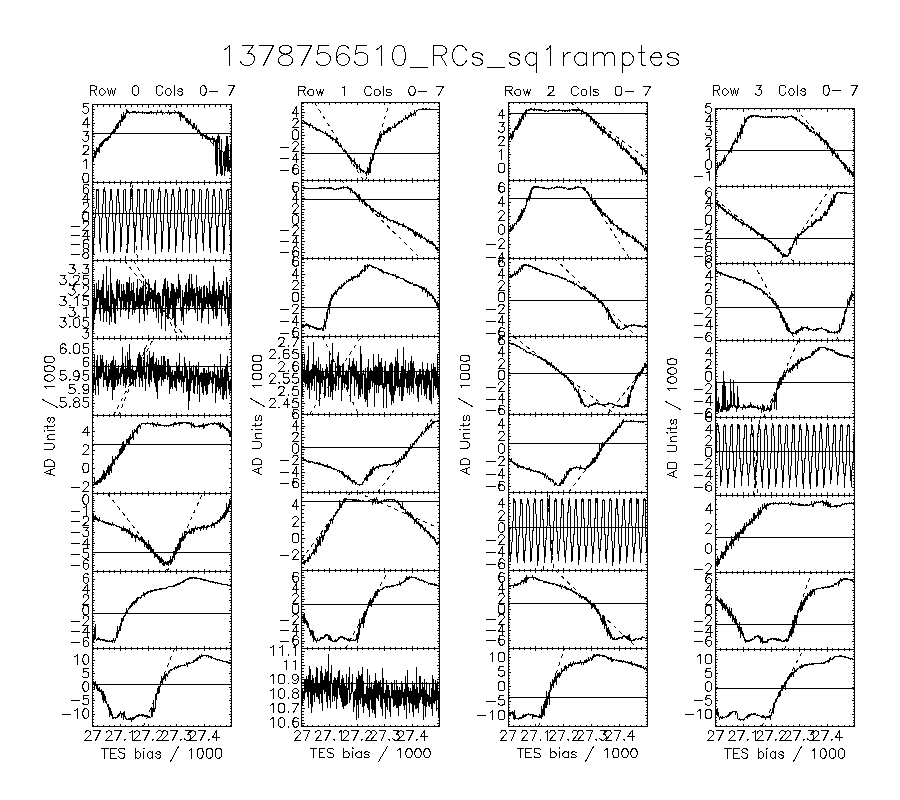
\includegraphics[width=\textwidth]{\here/../images/1378756510_RCs_sq1ramptes_00.png}
\caption{Plot showing response of SQUID amplifier chain to ramp in \TES\ bias current, while \TES\ is biased into transition. The change in applied bias current is the same as in \figref{fig:tes-bias-ramp-sc}.
Data is shown for rows 0--4 for all eight columns.
\RC{0}{2}, \RC{0}{3}, \RC{1}{3}, \RC{1}{7} all show no response, only noise (note the change in vertical scale for these row/columns).
\RC{0}{1}, \RC{2}{5} and \RC{3}{4} all respond as if they were still superconducting (see \figref{fig:tes-bias-ramp-sc}).
The much slower mapping of the $V$-$\phi$ curve indicates a much higher resistance in the \TES\ circuit loop, due to the \TES\ itself starting to go normal.
xxx need to explain units on axes?}
\label{fig:tes-bias-ramp-trans}
\end{figure*}

\begin{figure*}
\centering
\documentclass{standalone}

\usepackage{../thesis}

\usepackage{tikz} 
\usepackage{pgfplots} % drawing plots right here in this file!
\pgfplotsset{compat=1.9} % latest stable release

\usetikzlibrary{patterns}

\begin{document}
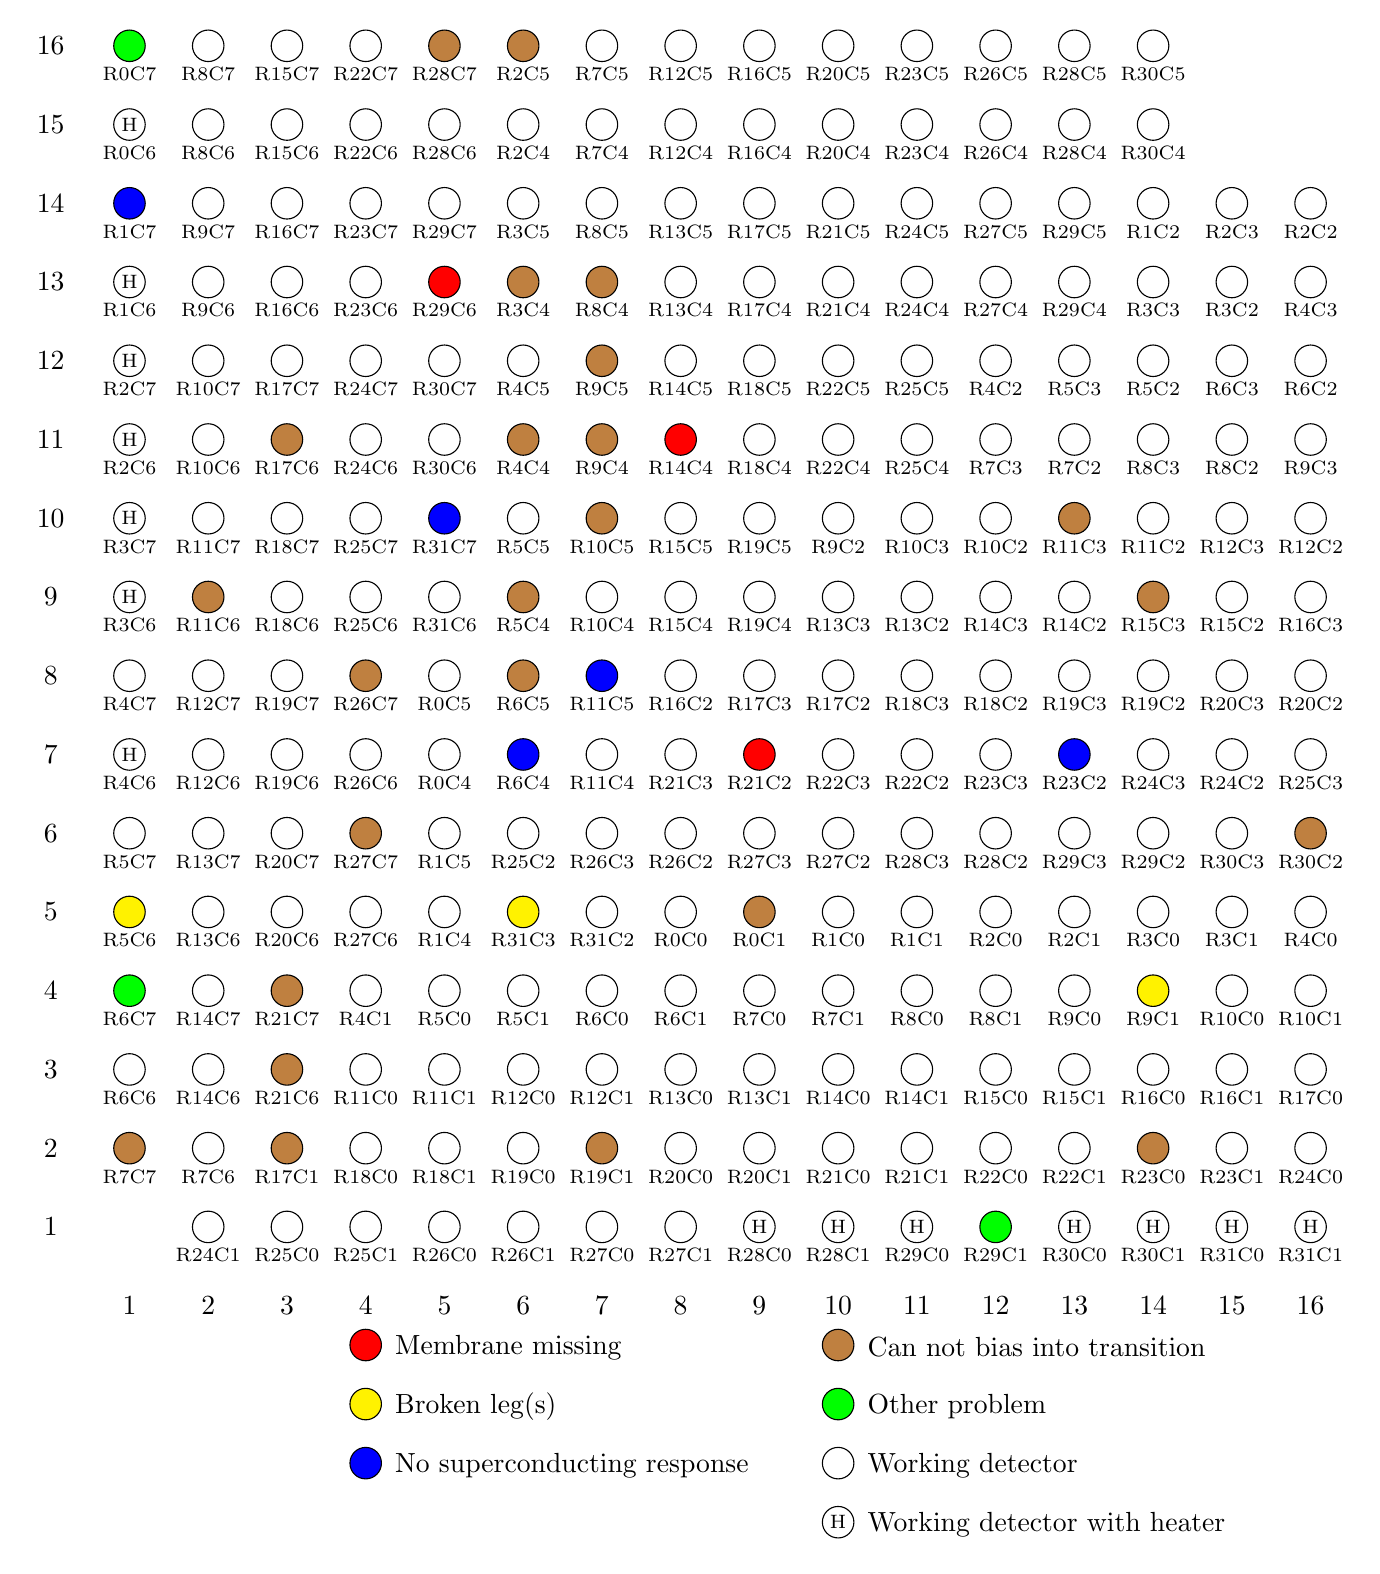
\begin{tikzpicture}
	
	%\pgfmathsetmacro{\d}{0.5}
	%\pgfmathsetmacro{\l}{2.0}
	%\pgfmathsetmacro{\D}{2}
	%\pgfmathsetmacro{\L}{2}
	%\pgfmathsetmacro{\phcy}{\l + \L - 0.5}
	%\pgfmathsetmacro{\phcy}{\l + \L - 0.5}

    \draw [fill=none] (8,5) circle [radius=0.2] node[font=\scriptsize] {} +(0,-0.15) node[below,font=\scriptsize] {R0C0};     \draw [fill=brown] (9,5) circle [radius=0.2] node[font=\scriptsize] {} +(0,-0.15) node[below,font=\scriptsize] {R0C1};     \draw [fill=none] (5,7) circle [radius=0.2] node[font=\scriptsize] {} +(0,-0.15) node[below,font=\scriptsize] {R0C4};     \draw [fill=none] (5,8) circle [radius=0.2] node[font=\scriptsize] {} +(0,-0.15) node[below,font=\scriptsize] {R0C5};     \draw [fill=none] (1,15) circle [radius=0.2] node[font=\scriptsize] {H} +(0,-0.15) node[below,font=\scriptsize] {R0C6};     \draw [fill=green] (1,16) circle [radius=0.2] node[font=\scriptsize] {} +(0,-0.15) node[below,font=\scriptsize] {R0C7}; 
    \draw [fill=none] (10,5) circle [radius=0.2] node[font=\scriptsize] {} +(0,-0.15) node[below,font=\scriptsize] {R1C0};     \draw [fill=none] (11,5) circle [radius=0.2] node[font=\scriptsize] {} +(0,-0.15) node[below,font=\scriptsize] {R1C1};     \draw [fill=none] (14,14) circle [radius=0.2] node[font=\scriptsize] {} +(0,-0.15) node[below,font=\scriptsize] {R1C2};     \draw [fill=none] (5,5) circle [radius=0.2] node[font=\scriptsize] {} +(0,-0.15) node[below,font=\scriptsize] {R1C4};     \draw [fill=none] (5,6) circle [radius=0.2] node[font=\scriptsize] {} +(0,-0.15) node[below,font=\scriptsize] {R1C5};     \draw [fill=none] (1,13) circle [radius=0.2] node[font=\scriptsize] {H} +(0,-0.15) node[below,font=\scriptsize] {R1C6};     \draw [fill=blue] (1,14) circle [radius=0.2] node[font=\scriptsize] {} +(0,-0.15) node[below,font=\scriptsize] {R1C7}; 
    \draw [fill=none] (12,5) circle [radius=0.2] node[font=\scriptsize] {} +(0,-0.15) node[below,font=\scriptsize] {R2C0};     \draw [fill=none] (13,5) circle [radius=0.2] node[font=\scriptsize] {} +(0,-0.15) node[below,font=\scriptsize] {R2C1};     \draw [fill=none] (16,14) circle [radius=0.2] node[font=\scriptsize] {} +(0,-0.15) node[below,font=\scriptsize] {R2C2};     \draw [fill=none] (15,14) circle [radius=0.2] node[font=\scriptsize] {} +(0,-0.15) node[below,font=\scriptsize] {R2C3};     \draw [fill=none] (6,15) circle [radius=0.2] node[font=\scriptsize] {} +(0,-0.15) node[below,font=\scriptsize] {R2C4};     \draw [fill=brown] (6,16) circle [radius=0.2] node[font=\scriptsize] {} +(0,-0.15) node[below,font=\scriptsize] {R2C5};     \draw [fill=none] (1,11) circle [radius=0.2] node[font=\scriptsize] {H} +(0,-0.15) node[below,font=\scriptsize] {R2C6};     \draw [fill=none] (1,12) circle [radius=0.2] node[font=\scriptsize] {H} +(0,-0.15) node[below,font=\scriptsize] {R2C7}; 
    \draw [fill=none] (14,5) circle [radius=0.2] node[font=\scriptsize] {} +(0,-0.15) node[below,font=\scriptsize] {R3C0};     \draw [fill=none] (15,5) circle [radius=0.2] node[font=\scriptsize] {} +(0,-0.15) node[below,font=\scriptsize] {R3C1};     \draw [fill=none] (15,13) circle [radius=0.2] node[font=\scriptsize] {} +(0,-0.15) node[below,font=\scriptsize] {R3C2};     \draw [fill=none] (14,13) circle [radius=0.2] node[font=\scriptsize] {} +(0,-0.15) node[below,font=\scriptsize] {R3C3};     \draw [fill=brown] (6,13) circle [radius=0.2] node[font=\scriptsize] {} +(0,-0.15) node[below,font=\scriptsize] {R3C4};     \draw [fill=none] (6,14) circle [radius=0.2] node[font=\scriptsize] {} +(0,-0.15) node[below,font=\scriptsize] {R3C5};     \draw [fill=none] (1,9) circle [radius=0.2] node[font=\scriptsize] {H} +(0,-0.15) node[below,font=\scriptsize] {R3C6};     \draw [fill=none] (1,10) circle [radius=0.2] node[font=\scriptsize] {H} +(0,-0.15) node[below,font=\scriptsize] {R3C7}; 
    \draw [fill=none] (16,5) circle [radius=0.2] node[font=\scriptsize] {} +(0,-0.15) node[below,font=\scriptsize] {R4C0};     \draw [fill=none] (4,4) circle [radius=0.2] node[font=\scriptsize] {} +(0,-0.15) node[below,font=\scriptsize] {R4C1};     \draw [fill=none] (12,12) circle [radius=0.2] node[font=\scriptsize] {} +(0,-0.15) node[below,font=\scriptsize] {R4C2};     \draw [fill=none] (16,13) circle [radius=0.2] node[font=\scriptsize] {} +(0,-0.15) node[below,font=\scriptsize] {R4C3};     \draw [fill=brown] (6,11) circle [radius=0.2] node[font=\scriptsize] {} +(0,-0.15) node[below,font=\scriptsize] {R4C4};     \draw [fill=none] (6,12) circle [radius=0.2] node[font=\scriptsize] {} +(0,-0.15) node[below,font=\scriptsize] {R4C5};     \draw [fill=none] (1,7) circle [radius=0.2] node[font=\scriptsize] {H} +(0,-0.15) node[below,font=\scriptsize] {R4C6};     \draw [fill=none] (1,8) circle [radius=0.2] node[font=\scriptsize] {} +(0,-0.15) node[below,font=\scriptsize] {R4C7}; 
    \draw [fill=none] (5,4) circle [radius=0.2] node[font=\scriptsize] {} +(0,-0.15) node[below,font=\scriptsize] {R5C0};     \draw [fill=none] (6,4) circle [radius=0.2] node[font=\scriptsize] {} +(0,-0.15) node[below,font=\scriptsize] {R5C1};     \draw [fill=none] (14,12) circle [radius=0.2] node[font=\scriptsize] {} +(0,-0.15) node[below,font=\scriptsize] {R5C2};     \draw [fill=none] (13,12) circle [radius=0.2] node[font=\scriptsize] {} +(0,-0.15) node[below,font=\scriptsize] {R5C3};     \draw [fill=brown] (6,9) circle [radius=0.2] node[font=\scriptsize] {} +(0,-0.15) node[below,font=\scriptsize] {R5C4};     \draw [fill=none] (6,10) circle [radius=0.2] node[font=\scriptsize] {} +(0,-0.15) node[below,font=\scriptsize] {R5C5};     \draw [fill=yellow] (1,5) circle [radius=0.2] node[font=\scriptsize] {} +(0,-0.15) node[below,font=\scriptsize] {R5C6};     \draw [fill=none] (1,6) circle [radius=0.2] node[font=\scriptsize] {} +(0,-0.15) node[below,font=\scriptsize] {R5C7}; 
    \draw [fill=none] (7,4) circle [radius=0.2] node[font=\scriptsize] {} +(0,-0.15) node[below,font=\scriptsize] {R6C0};     \draw [fill=none] (8,4) circle [radius=0.2] node[font=\scriptsize] {} +(0,-0.15) node[below,font=\scriptsize] {R6C1};     \draw [fill=none] (16,12) circle [radius=0.2] node[font=\scriptsize] {} +(0,-0.15) node[below,font=\scriptsize] {R6C2};     \draw [fill=none] (15,12) circle [radius=0.2] node[font=\scriptsize] {} +(0,-0.15) node[below,font=\scriptsize] {R6C3};     \draw [fill=blue] (6,7) circle [radius=0.2] node[font=\scriptsize] {} +(0,-0.15) node[below,font=\scriptsize] {R6C4};     \draw [fill=brown] (6,8) circle [radius=0.2] node[font=\scriptsize] {} +(0,-0.15) node[below,font=\scriptsize] {R6C5};     \draw [fill=none] (1,3) circle [radius=0.2] node[font=\scriptsize] {} +(0,-0.15) node[below,font=\scriptsize] {R6C6};     \draw [fill=green] (1,4) circle [radius=0.2] node[font=\scriptsize] {} +(0,-0.15) node[below,font=\scriptsize] {R6C7}; 
    \draw [fill=none] (9,4) circle [radius=0.2] node[font=\scriptsize] {} +(0,-0.15) node[below,font=\scriptsize] {R7C0};     \draw [fill=none] (10,4) circle [radius=0.2] node[font=\scriptsize] {} +(0,-0.15) node[below,font=\scriptsize] {R7C1};     \draw [fill=none] (13,11) circle [radius=0.2] node[font=\scriptsize] {} +(0,-0.15) node[below,font=\scriptsize] {R7C2};     \draw [fill=none] (12,11) circle [radius=0.2] node[font=\scriptsize] {} +(0,-0.15) node[below,font=\scriptsize] {R7C3};     \draw [fill=none] (7,15) circle [radius=0.2] node[font=\scriptsize] {} +(0,-0.15) node[below,font=\scriptsize] {R7C4};     \draw [fill=none] (7,16) circle [radius=0.2] node[font=\scriptsize] {} +(0,-0.15) node[below,font=\scriptsize] {R7C5};     \draw [fill=none] (2,2) circle [radius=0.2] node[font=\scriptsize] {} +(0,-0.15) node[below,font=\scriptsize] {R7C6};     \draw [fill=brown] (1,2) circle [radius=0.2] node[font=\scriptsize] {} +(0,-0.15) node[below,font=\scriptsize] {R7C7}; 
    \draw [fill=none] (11,4) circle [radius=0.2] node[font=\scriptsize] {} +(0,-0.15) node[below,font=\scriptsize] {R8C0};     \draw [fill=none] (12,4) circle [radius=0.2] node[font=\scriptsize] {} +(0,-0.15) node[below,font=\scriptsize] {R8C1};     \draw [fill=none] (15,11) circle [radius=0.2] node[font=\scriptsize] {} +(0,-0.15) node[below,font=\scriptsize] {R8C2};     \draw [fill=none] (14,11) circle [radius=0.2] node[font=\scriptsize] {} +(0,-0.15) node[below,font=\scriptsize] {R8C3};     \draw [fill=brown] (7,13) circle [radius=0.2] node[font=\scriptsize] {} +(0,-0.15) node[below,font=\scriptsize] {R8C4};     \draw [fill=none] (7,14) circle [radius=0.2] node[font=\scriptsize] {} +(0,-0.15) node[below,font=\scriptsize] {R8C5};     \draw [fill=none] (2,15) circle [radius=0.2] node[font=\scriptsize] {} +(0,-0.15) node[below,font=\scriptsize] {R8C6};     \draw [fill=none] (2,16) circle [radius=0.2] node[font=\scriptsize] {} +(0,-0.15) node[below,font=\scriptsize] {R8C7}; 
    \draw [fill=none] (13,4) circle [radius=0.2] node[font=\scriptsize] {} +(0,-0.15) node[below,font=\scriptsize] {R9C0};     \draw [fill=yellow] (14,4) circle [radius=0.2] node[font=\scriptsize] {} +(0,-0.15) node[below,font=\scriptsize] {R9C1};     \draw [fill=none] (10,10) circle [radius=0.2] node[font=\scriptsize] {} +(0,-0.15) node[below,font=\scriptsize] {R9C2};     \draw [fill=none] (16,11) circle [radius=0.2] node[font=\scriptsize] {} +(0,-0.15) node[below,font=\scriptsize] {R9C3};     \draw [fill=brown] (7,11) circle [radius=0.2] node[font=\scriptsize] {} +(0,-0.15) node[below,font=\scriptsize] {R9C4};     \draw [fill=brown] (7,12) circle [radius=0.2] node[font=\scriptsize] {} +(0,-0.15) node[below,font=\scriptsize] {R9C5};     \draw [fill=none] (2,13) circle [radius=0.2] node[font=\scriptsize] {} +(0,-0.15) node[below,font=\scriptsize] {R9C6};     \draw [fill=none] (2,14) circle [radius=0.2] node[font=\scriptsize] {} +(0,-0.15) node[below,font=\scriptsize] {R9C7}; 
    \draw [fill=none] (15,4) circle [radius=0.2] node[font=\scriptsize] {} +(0,-0.15) node[below,font=\scriptsize] {R10C0};     \draw [fill=none] (16,4) circle [radius=0.2] node[font=\scriptsize] {} +(0,-0.15) node[below,font=\scriptsize] {R10C1};     \draw [fill=none] (12,10) circle [radius=0.2] node[font=\scriptsize] {} +(0,-0.15) node[below,font=\scriptsize] {R10C2};     \draw [fill=none] (11,10) circle [radius=0.2] node[font=\scriptsize] {} +(0,-0.15) node[below,font=\scriptsize] {R10C3};     \draw [fill=none] (7,9) circle [radius=0.2] node[font=\scriptsize] {} +(0,-0.15) node[below,font=\scriptsize] {R10C4};     \draw [fill=brown] (7,10) circle [radius=0.2] node[font=\scriptsize] {} +(0,-0.15) node[below,font=\scriptsize] {R10C5};     \draw [fill=none] (2,11) circle [radius=0.2] node[font=\scriptsize] {} +(0,-0.15) node[below,font=\scriptsize] {R10C6};     \draw [fill=none] (2,12) circle [radius=0.2] node[font=\scriptsize] {} +(0,-0.15) node[below,font=\scriptsize] {R10C7}; 
    \draw [fill=none] (4,3) circle [radius=0.2] node[font=\scriptsize] {} +(0,-0.15) node[below,font=\scriptsize] {R11C0};     \draw [fill=none] (5,3) circle [radius=0.2] node[font=\scriptsize] {} +(0,-0.15) node[below,font=\scriptsize] {R11C1};     \draw [fill=none] (14,10) circle [radius=0.2] node[font=\scriptsize] {} +(0,-0.15) node[below,font=\scriptsize] {R11C2};     \draw [fill=brown] (13,10) circle [radius=0.2] node[font=\scriptsize] {} +(0,-0.15) node[below,font=\scriptsize] {R11C3};     \draw [fill=none] (7,7) circle [radius=0.2] node[font=\scriptsize] {} +(0,-0.15) node[below,font=\scriptsize] {R11C4};     \draw [fill=blue] (7,8) circle [radius=0.2] node[font=\scriptsize] {} +(0,-0.15) node[below,font=\scriptsize] {R11C5};     \draw [fill=brown] (2,9) circle [radius=0.2] node[font=\scriptsize] {} +(0,-0.15) node[below,font=\scriptsize] {R11C6};     \draw [fill=none] (2,10) circle [radius=0.2] node[font=\scriptsize] {} +(0,-0.15) node[below,font=\scriptsize] {R11C7}; 
    \draw [fill=none] (6,3) circle [radius=0.2] node[font=\scriptsize] {} +(0,-0.15) node[below,font=\scriptsize] {R12C0};     \draw [fill=none] (7,3) circle [radius=0.2] node[font=\scriptsize] {} +(0,-0.15) node[below,font=\scriptsize] {R12C1};     \draw [fill=none] (16,10) circle [radius=0.2] node[font=\scriptsize] {} +(0,-0.15) node[below,font=\scriptsize] {R12C2};     \draw [fill=none] (15,10) circle [radius=0.2] node[font=\scriptsize] {} +(0,-0.15) node[below,font=\scriptsize] {R12C3};     \draw [fill=none] (8,15) circle [radius=0.2] node[font=\scriptsize] {} +(0,-0.15) node[below,font=\scriptsize] {R12C4};     \draw [fill=none] (8,16) circle [radius=0.2] node[font=\scriptsize] {} +(0,-0.15) node[below,font=\scriptsize] {R12C5};     \draw [fill=none] (2,7) circle [radius=0.2] node[font=\scriptsize] {} +(0,-0.15) node[below,font=\scriptsize] {R12C6};     \draw [fill=none] (2,8) circle [radius=0.2] node[font=\scriptsize] {} +(0,-0.15) node[below,font=\scriptsize] {R12C7}; 
    \draw [fill=none] (8,3) circle [radius=0.2] node[font=\scriptsize] {} +(0,-0.15) node[below,font=\scriptsize] {R13C0};     \draw [fill=none] (9,3) circle [radius=0.2] node[font=\scriptsize] {} +(0,-0.15) node[below,font=\scriptsize] {R13C1};     \draw [fill=none] (11,9) circle [radius=0.2] node[font=\scriptsize] {} +(0,-0.15) node[below,font=\scriptsize] {R13C2};     \draw [fill=none] (10,9) circle [radius=0.2] node[font=\scriptsize] {} +(0,-0.15) node[below,font=\scriptsize] {R13C3};     \draw [fill=none] (8,13) circle [radius=0.2] node[font=\scriptsize] {} +(0,-0.15) node[below,font=\scriptsize] {R13C4};     \draw [fill=none] (8,14) circle [radius=0.2] node[font=\scriptsize] {} +(0,-0.15) node[below,font=\scriptsize] {R13C5};     \draw [fill=none] (2,5) circle [radius=0.2] node[font=\scriptsize] {} +(0,-0.15) node[below,font=\scriptsize] {R13C6};     \draw [fill=none] (2,6) circle [radius=0.2] node[font=\scriptsize] {} +(0,-0.15) node[below,font=\scriptsize] {R13C7}; 
    \draw [fill=none] (10,3) circle [radius=0.2] node[font=\scriptsize] {} +(0,-0.15) node[below,font=\scriptsize] {R14C0};     \draw [fill=none] (11,3) circle [radius=0.2] node[font=\scriptsize] {} +(0,-0.15) node[below,font=\scriptsize] {R14C1};     \draw [fill=none] (13,9) circle [radius=0.2] node[font=\scriptsize] {} +(0,-0.15) node[below,font=\scriptsize] {R14C2};     \draw [fill=none] (12,9) circle [radius=0.2] node[font=\scriptsize] {} +(0,-0.15) node[below,font=\scriptsize] {R14C3};     \draw [fill=red] (8,11) circle [radius=0.2] node[font=\scriptsize] {} +(0,-0.15) node[below,font=\scriptsize] {R14C4};     \draw [fill=none] (8,12) circle [radius=0.2] node[font=\scriptsize] {} +(0,-0.15) node[below,font=\scriptsize] {R14C5};     \draw [fill=none] (2,3) circle [radius=0.2] node[font=\scriptsize] {} +(0,-0.15) node[below,font=\scriptsize] {R14C6};     \draw [fill=none] (2,4) circle [radius=0.2] node[font=\scriptsize] {} +(0,-0.15) node[below,font=\scriptsize] {R14C7}; 
    \draw [fill=none] (12,3) circle [radius=0.2] node[font=\scriptsize] {} +(0,-0.15) node[below,font=\scriptsize] {R15C0};     \draw [fill=none] (13,3) circle [radius=0.2] node[font=\scriptsize] {} +(0,-0.15) node[below,font=\scriptsize] {R15C1};     \draw [fill=none] (15,9) circle [radius=0.2] node[font=\scriptsize] {} +(0,-0.15) node[below,font=\scriptsize] {R15C2};     \draw [fill=brown] (14,9) circle [radius=0.2] node[font=\scriptsize] {} +(0,-0.15) node[below,font=\scriptsize] {R15C3};     \draw [fill=none] (8,9) circle [radius=0.2] node[font=\scriptsize] {} +(0,-0.15) node[below,font=\scriptsize] {R15C4};     \draw [fill=none] (8,10) circle [radius=0.2] node[font=\scriptsize] {} +(0,-0.15) node[below,font=\scriptsize] {R15C5};     \draw [fill=none] (3,15) circle [radius=0.2] node[font=\scriptsize] {} +(0,-0.15) node[below,font=\scriptsize] {R15C6};     \draw [fill=none] (3,16) circle [radius=0.2] node[font=\scriptsize] {} +(0,-0.15) node[below,font=\scriptsize] {R15C7}; 
    \draw [fill=none] (14,3) circle [radius=0.2] node[font=\scriptsize] {} +(0,-0.15) node[below,font=\scriptsize] {R16C0};     \draw [fill=none] (15,3) circle [radius=0.2] node[font=\scriptsize] {} +(0,-0.15) node[below,font=\scriptsize] {R16C1};     \draw [fill=none] (8,8) circle [radius=0.2] node[font=\scriptsize] {} +(0,-0.15) node[below,font=\scriptsize] {R16C2};     \draw [fill=none] (16,9) circle [radius=0.2] node[font=\scriptsize] {} +(0,-0.15) node[below,font=\scriptsize] {R16C3};     \draw [fill=none] (9,15) circle [radius=0.2] node[font=\scriptsize] {} +(0,-0.15) node[below,font=\scriptsize] {R16C4};     \draw [fill=none] (9,16) circle [radius=0.2] node[font=\scriptsize] {} +(0,-0.15) node[below,font=\scriptsize] {R16C5};     \draw [fill=none] (3,13) circle [radius=0.2] node[font=\scriptsize] {} +(0,-0.15) node[below,font=\scriptsize] {R16C6};     \draw [fill=none] (3,14) circle [radius=0.2] node[font=\scriptsize] {} +(0,-0.15) node[below,font=\scriptsize] {R16C7}; 
    \draw [fill=none] (16,3) circle [radius=0.2] node[font=\scriptsize] {} +(0,-0.15) node[below,font=\scriptsize] {R17C0};     \draw [fill=brown] (3,2) circle [radius=0.2] node[font=\scriptsize] {} +(0,-0.15) node[below,font=\scriptsize] {R17C1};     \draw [fill=none] (10,8) circle [radius=0.2] node[font=\scriptsize] {} +(0,-0.15) node[below,font=\scriptsize] {R17C2};     \draw [fill=none] (9,8) circle [radius=0.2] node[font=\scriptsize] {} +(0,-0.15) node[below,font=\scriptsize] {R17C3};     \draw [fill=none] (9,13) circle [radius=0.2] node[font=\scriptsize] {} +(0,-0.15) node[below,font=\scriptsize] {R17C4};     \draw [fill=none] (9,14) circle [radius=0.2] node[font=\scriptsize] {} +(0,-0.15) node[below,font=\scriptsize] {R17C5};     \draw [fill=brown] (3,11) circle [radius=0.2] node[font=\scriptsize] {} +(0,-0.15) node[below,font=\scriptsize] {R17C6};     \draw [fill=none] (3,12) circle [radius=0.2] node[font=\scriptsize] {} +(0,-0.15) node[below,font=\scriptsize] {R17C7}; 
    \draw [fill=none] (4,2) circle [radius=0.2] node[font=\scriptsize] {} +(0,-0.15) node[below,font=\scriptsize] {R18C0};     \draw [fill=none] (5,2) circle [radius=0.2] node[font=\scriptsize] {} +(0,-0.15) node[below,font=\scriptsize] {R18C1};     \draw [fill=none] (12,8) circle [radius=0.2] node[font=\scriptsize] {} +(0,-0.15) node[below,font=\scriptsize] {R18C2};     \draw [fill=none] (11,8) circle [radius=0.2] node[font=\scriptsize] {} +(0,-0.15) node[below,font=\scriptsize] {R18C3};     \draw [fill=none] (9,11) circle [radius=0.2] node[font=\scriptsize] {} +(0,-0.15) node[below,font=\scriptsize] {R18C4};     \draw [fill=none] (9,12) circle [radius=0.2] node[font=\scriptsize] {} +(0,-0.15) node[below,font=\scriptsize] {R18C5};     \draw [fill=none] (3,9) circle [radius=0.2] node[font=\scriptsize] {} +(0,-0.15) node[below,font=\scriptsize] {R18C6};     \draw [fill=none] (3,10) circle [radius=0.2] node[font=\scriptsize] {} +(0,-0.15) node[below,font=\scriptsize] {R18C7}; 
    \draw [fill=none] (6,2) circle [radius=0.2] node[font=\scriptsize] {} +(0,-0.15) node[below,font=\scriptsize] {R19C0};     \draw [fill=brown] (7,2) circle [radius=0.2] node[font=\scriptsize] {} +(0,-0.15) node[below,font=\scriptsize] {R19C1};     \draw [fill=none] (14,8) circle [radius=0.2] node[font=\scriptsize] {} +(0,-0.15) node[below,font=\scriptsize] {R19C2};     \draw [fill=none] (13,8) circle [radius=0.2] node[font=\scriptsize] {} +(0,-0.15) node[below,font=\scriptsize] {R19C3};     \draw [fill=none] (9,9) circle [radius=0.2] node[font=\scriptsize] {} +(0,-0.15) node[below,font=\scriptsize] {R19C4};     \draw [fill=none] (9,10) circle [radius=0.2] node[font=\scriptsize] {} +(0,-0.15) node[below,font=\scriptsize] {R19C5};     \draw [fill=none] (3,7) circle [radius=0.2] node[font=\scriptsize] {} +(0,-0.15) node[below,font=\scriptsize] {R19C6};     \draw [fill=none] (3,8) circle [radius=0.2] node[font=\scriptsize] {} +(0,-0.15) node[below,font=\scriptsize] {R19C7}; 
    \draw [fill=none] (8,2) circle [radius=0.2] node[font=\scriptsize] {} +(0,-0.15) node[below,font=\scriptsize] {R20C0};     \draw [fill=none] (9,2) circle [radius=0.2] node[font=\scriptsize] {} +(0,-0.15) node[below,font=\scriptsize] {R20C1};     \draw [fill=none] (16,8) circle [radius=0.2] node[font=\scriptsize] {} +(0,-0.15) node[below,font=\scriptsize] {R20C2};     \draw [fill=none] (15,8) circle [radius=0.2] node[font=\scriptsize] {} +(0,-0.15) node[below,font=\scriptsize] {R20C3};     \draw [fill=none] (10,15) circle [radius=0.2] node[font=\scriptsize] {} +(0,-0.15) node[below,font=\scriptsize] {R20C4};     \draw [fill=none] (10,16) circle [radius=0.2] node[font=\scriptsize] {} +(0,-0.15) node[below,font=\scriptsize] {R20C5};     \draw [fill=none] (3,5) circle [radius=0.2] node[font=\scriptsize] {} +(0,-0.15) node[below,font=\scriptsize] {R20C6};     \draw [fill=none] (3,6) circle [radius=0.2] node[font=\scriptsize] {} +(0,-0.15) node[below,font=\scriptsize] {R20C7}; 
    \draw [fill=none] (10,2) circle [radius=0.2] node[font=\scriptsize] {} +(0,-0.15) node[below,font=\scriptsize] {R21C0};     \draw [fill=none] (11,2) circle [radius=0.2] node[font=\scriptsize] {} +(0,-0.15) node[below,font=\scriptsize] {R21C1};     \draw [fill=red] (9,7) circle [radius=0.2] node[font=\scriptsize] {} +(0,-0.15) node[below,font=\scriptsize] {R21C2};     \draw [fill=none] (8,7) circle [radius=0.2] node[font=\scriptsize] {} +(0,-0.15) node[below,font=\scriptsize] {R21C3};     \draw [fill=none] (10,13) circle [radius=0.2] node[font=\scriptsize] {} +(0,-0.15) node[below,font=\scriptsize] {R21C4};     \draw [fill=none] (10,14) circle [radius=0.2] node[font=\scriptsize] {} +(0,-0.15) node[below,font=\scriptsize] {R21C5};     \draw [fill=brown] (3,3) circle [radius=0.2] node[font=\scriptsize] {} +(0,-0.15) node[below,font=\scriptsize] {R21C6};     \draw [fill=brown] (3,4) circle [radius=0.2] node[font=\scriptsize] {} +(0,-0.15) node[below,font=\scriptsize] {R21C7}; 
    \draw [fill=none] (12,2) circle [radius=0.2] node[font=\scriptsize] {} +(0,-0.15) node[below,font=\scriptsize] {R22C0};     \draw [fill=none] (13,2) circle [radius=0.2] node[font=\scriptsize] {} +(0,-0.15) node[below,font=\scriptsize] {R22C1};     \draw [fill=none] (11,7) circle [radius=0.2] node[font=\scriptsize] {} +(0,-0.15) node[below,font=\scriptsize] {R22C2};     \draw [fill=none] (10,7) circle [radius=0.2] node[font=\scriptsize] {} +(0,-0.15) node[below,font=\scriptsize] {R22C3};     \draw [fill=none] (10,11) circle [radius=0.2] node[font=\scriptsize] {} +(0,-0.15) node[below,font=\scriptsize] {R22C4};     \draw [fill=none] (10,12) circle [radius=0.2] node[font=\scriptsize] {} +(0,-0.15) node[below,font=\scriptsize] {R22C5};     \draw [fill=none] (4,15) circle [radius=0.2] node[font=\scriptsize] {} +(0,-0.15) node[below,font=\scriptsize] {R22C6};     \draw [fill=none] (4,16) circle [radius=0.2] node[font=\scriptsize] {} +(0,-0.15) node[below,font=\scriptsize] {R22C7}; 
    \draw [fill=brown] (14,2) circle [radius=0.2] node[font=\scriptsize] {} +(0,-0.15) node[below,font=\scriptsize] {R23C0};     \draw [fill=none] (15,2) circle [radius=0.2] node[font=\scriptsize] {} +(0,-0.15) node[below,font=\scriptsize] {R23C1};     \draw [fill=blue] (13,7) circle [radius=0.2] node[font=\scriptsize] {} +(0,-0.15) node[below,font=\scriptsize] {R23C2};     \draw [fill=none] (12,7) circle [radius=0.2] node[font=\scriptsize] {} +(0,-0.15) node[below,font=\scriptsize] {R23C3};     \draw [fill=none] (11,15) circle [radius=0.2] node[font=\scriptsize] {} +(0,-0.15) node[below,font=\scriptsize] {R23C4};     \draw [fill=none] (11,16) circle [radius=0.2] node[font=\scriptsize] {} +(0,-0.15) node[below,font=\scriptsize] {R23C5};     \draw [fill=none] (4,13) circle [radius=0.2] node[font=\scriptsize] {} +(0,-0.15) node[below,font=\scriptsize] {R23C6};     \draw [fill=none] (4,14) circle [radius=0.2] node[font=\scriptsize] {} +(0,-0.15) node[below,font=\scriptsize] {R23C7}; 
    \draw [fill=none] (16,2) circle [radius=0.2] node[font=\scriptsize] {} +(0,-0.15) node[below,font=\scriptsize] {R24C0};     \draw [fill=none] (2,1) circle [radius=0.2] node[font=\scriptsize] {} +(0,-0.15) node[below,font=\scriptsize] {R24C1};     \draw [fill=none] (15,7) circle [radius=0.2] node[font=\scriptsize] {} +(0,-0.15) node[below,font=\scriptsize] {R24C2};     \draw [fill=none] (14,7) circle [radius=0.2] node[font=\scriptsize] {} +(0,-0.15) node[below,font=\scriptsize] {R24C3};     \draw [fill=none] (11,13) circle [radius=0.2] node[font=\scriptsize] {} +(0,-0.15) node[below,font=\scriptsize] {R24C4};     \draw [fill=none] (11,14) circle [radius=0.2] node[font=\scriptsize] {} +(0,-0.15) node[below,font=\scriptsize] {R24C5};     \draw [fill=none] (4,11) circle [radius=0.2] node[font=\scriptsize] {} +(0,-0.15) node[below,font=\scriptsize] {R24C6};     \draw [fill=none] (4,12) circle [radius=0.2] node[font=\scriptsize] {} +(0,-0.15) node[below,font=\scriptsize] {R24C7}; 
    \draw [fill=none] (3,1) circle [radius=0.2] node[font=\scriptsize] {} +(0,-0.15) node[below,font=\scriptsize] {R25C0};     \draw [fill=none] (4,1) circle [radius=0.2] node[font=\scriptsize] {} +(0,-0.15) node[below,font=\scriptsize] {R25C1};     \draw [fill=none] (6,6) circle [radius=0.2] node[font=\scriptsize] {} +(0,-0.15) node[below,font=\scriptsize] {R25C2};     \draw [fill=none] (16,7) circle [radius=0.2] node[font=\scriptsize] {} +(0,-0.15) node[below,font=\scriptsize] {R25C3};     \draw [fill=none] (11,11) circle [radius=0.2] node[font=\scriptsize] {} +(0,-0.15) node[below,font=\scriptsize] {R25C4};     \draw [fill=none] (11,12) circle [radius=0.2] node[font=\scriptsize] {} +(0,-0.15) node[below,font=\scriptsize] {R25C5};     \draw [fill=none] (4,9) circle [radius=0.2] node[font=\scriptsize] {} +(0,-0.15) node[below,font=\scriptsize] {R25C6};     \draw [fill=none] (4,10) circle [radius=0.2] node[font=\scriptsize] {} +(0,-0.15) node[below,font=\scriptsize] {R25C7}; 
    \draw [fill=none] (5,1) circle [radius=0.2] node[font=\scriptsize] {} +(0,-0.15) node[below,font=\scriptsize] {R26C0};     \draw [fill=none] (6,1) circle [radius=0.2] node[font=\scriptsize] {} +(0,-0.15) node[below,font=\scriptsize] {R26C1};     \draw [fill=none] (8,6) circle [radius=0.2] node[font=\scriptsize] {} +(0,-0.15) node[below,font=\scriptsize] {R26C2};     \draw [fill=none] (7,6) circle [radius=0.2] node[font=\scriptsize] {} +(0,-0.15) node[below,font=\scriptsize] {R26C3};     \draw [fill=none] (12,15) circle [radius=0.2] node[font=\scriptsize] {} +(0,-0.15) node[below,font=\scriptsize] {R26C4};     \draw [fill=none] (12,16) circle [radius=0.2] node[font=\scriptsize] {} +(0,-0.15) node[below,font=\scriptsize] {R26C5};     \draw [fill=none] (4,7) circle [radius=0.2] node[font=\scriptsize] {} +(0,-0.15) node[below,font=\scriptsize] {R26C6};     \draw [fill=brown] (4,8) circle [radius=0.2] node[font=\scriptsize] {} +(0,-0.15) node[below,font=\scriptsize] {R26C7}; 
    \draw [fill=none] (7,1) circle [radius=0.2] node[font=\scriptsize] {} +(0,-0.15) node[below,font=\scriptsize] {R27C0};     \draw [fill=none] (8,1) circle [radius=0.2] node[font=\scriptsize] {} +(0,-0.15) node[below,font=\scriptsize] {R27C1};     \draw [fill=none] (10,6) circle [radius=0.2] node[font=\scriptsize] {} +(0,-0.15) node[below,font=\scriptsize] {R27C2};     \draw [fill=none] (9,6) circle [radius=0.2] node[font=\scriptsize] {} +(0,-0.15) node[below,font=\scriptsize] {R27C3};     \draw [fill=none] (12,13) circle [radius=0.2] node[font=\scriptsize] {} +(0,-0.15) node[below,font=\scriptsize] {R27C4};     \draw [fill=none] (12,14) circle [radius=0.2] node[font=\scriptsize] {} +(0,-0.15) node[below,font=\scriptsize] {R27C5};     \draw [fill=none] (4,5) circle [radius=0.2] node[font=\scriptsize] {} +(0,-0.15) node[below,font=\scriptsize] {R27C6};     \draw [fill=brown] (4,6) circle [radius=0.2] node[font=\scriptsize] {} +(0,-0.15) node[below,font=\scriptsize] {R27C7}; 
    \draw [fill=none] (9,1) circle [radius=0.2] node[font=\scriptsize] {H} +(0,-0.15) node[below,font=\scriptsize] {R28C0};     \draw [fill=none] (10,1) circle [radius=0.2] node[font=\scriptsize] {H} +(0,-0.15) node[below,font=\scriptsize] {R28C1};     \draw [fill=none] (12,6) circle [radius=0.2] node[font=\scriptsize] {} +(0,-0.15) node[below,font=\scriptsize] {R28C2};     \draw [fill=none] (11,6) circle [radius=0.2] node[font=\scriptsize] {} +(0,-0.15) node[below,font=\scriptsize] {R28C3};     \draw [fill=none] (13,15) circle [radius=0.2] node[font=\scriptsize] {} +(0,-0.15) node[below,font=\scriptsize] {R28C4};     \draw [fill=none] (13,16) circle [radius=0.2] node[font=\scriptsize] {} +(0,-0.15) node[below,font=\scriptsize] {R28C5};     \draw [fill=none] (5,15) circle [radius=0.2] node[font=\scriptsize] {} +(0,-0.15) node[below,font=\scriptsize] {R28C6};     \draw [fill=brown] (5,16) circle [radius=0.2] node[font=\scriptsize] {} +(0,-0.15) node[below,font=\scriptsize] {R28C7}; 
    \draw [fill=none] (11,1) circle [radius=0.2] node[font=\scriptsize] {H} +(0,-0.15) node[below,font=\scriptsize] {R29C0};     \draw [fill=green] (12,1) circle [radius=0.2] node[font=\scriptsize] {} +(0,-0.15) node[below,font=\scriptsize] {R29C1};     \draw [fill=none] (14,6) circle [radius=0.2] node[font=\scriptsize] {} +(0,-0.15) node[below,font=\scriptsize] {R29C2};     \draw [fill=none] (13,6) circle [radius=0.2] node[font=\scriptsize] {} +(0,-0.15) node[below,font=\scriptsize] {R29C3};     \draw [fill=none] (13,13) circle [radius=0.2] node[font=\scriptsize] {} +(0,-0.15) node[below,font=\scriptsize] {R29C4};     \draw [fill=none] (13,14) circle [radius=0.2] node[font=\scriptsize] {} +(0,-0.15) node[below,font=\scriptsize] {R29C5};     \draw [fill=red] (5,13) circle [radius=0.2] node[font=\scriptsize] {} +(0,-0.15) node[below,font=\scriptsize] {R29C6};     \draw [fill=none] (5,14) circle [radius=0.2] node[font=\scriptsize] {} +(0,-0.15) node[below,font=\scriptsize] {R29C7}; 
    \draw [fill=none] (13,1) circle [radius=0.2] node[font=\scriptsize] {H} +(0,-0.15) node[below,font=\scriptsize] {R30C0};     \draw [fill=none] (14,1) circle [radius=0.2] node[font=\scriptsize] {H} +(0,-0.15) node[below,font=\scriptsize] {R30C1};     \draw [fill=brown] (16,6) circle [radius=0.2] node[font=\scriptsize] {} +(0,-0.15) node[below,font=\scriptsize] {R30C2};     \draw [fill=none] (15,6) circle [radius=0.2] node[font=\scriptsize] {} +(0,-0.15) node[below,font=\scriptsize] {R30C3};     \draw [fill=none] (14,15) circle [radius=0.2] node[font=\scriptsize] {} +(0,-0.15) node[below,font=\scriptsize] {R30C4};     \draw [fill=none] (14,16) circle [radius=0.2] node[font=\scriptsize] {} +(0,-0.15) node[below,font=\scriptsize] {R30C5};     \draw [fill=none] (5,11) circle [radius=0.2] node[font=\scriptsize] {} +(0,-0.15) node[below,font=\scriptsize] {R30C6};     \draw [fill=none] (5,12) circle [radius=0.2] node[font=\scriptsize] {} +(0,-0.15) node[below,font=\scriptsize] {R30C7}; 
    \draw [fill=none] (15,1) circle [radius=0.2] node[font=\scriptsize] {H} +(0,-0.15) node[below,font=\scriptsize] {R31C0};     \draw [fill=none] (16,1) circle [radius=0.2] node[font=\scriptsize] {H} +(0,-0.15) node[below,font=\scriptsize] {R31C1};     \draw [fill=none] (7,5) circle [radius=0.2] node[font=\scriptsize] {} +(0,-0.15) node[below,font=\scriptsize] {R31C2};     \draw [fill=yellow] (6,5) circle [radius=0.2] node[font=\scriptsize] {} +(0,-0.15) node[below,font=\scriptsize] {R31C3};     \draw [fill=none] (5,9) circle [radius=0.2] node[font=\scriptsize] {} +(0,-0.15) node[below,font=\scriptsize] {R31C6};     \draw [fill=blue] (5,10) circle [radius=0.2] node[font=\scriptsize] {} +(0,-0.15) node[below,font=\scriptsize] {R31C7}; 

	% detector labels
	\foreach \x in {1,...,16} \draw (\x, 0) node {\x};
	\foreach \y in {1,...,16} \draw (0, \y) node {\y};

	% legend
	\draw [fill=red] (4,-0.5) circle [radius=0.2] +(0.25,-0.03) node[right] {Membrane missing};
	\draw [fill=yellow] (4,-1.25) circle [radius=0.2] +(0.25,-0.03) node[right] {Broken leg(s)};
	\draw [fill=blue] (4,-2.0) circle [radius=0.2] +(0.25,-0.03) node[right] {No superconducting response};
	\draw [fill=brown] (10,-0.5) circle [radius=0.2] +(0.25,-0.03) node[right] {Can not bias into transition};
	\draw [fill=green] (10,-1.25) circle [radius=0.2] +(0.25,-0.03) node[right] {Other problem};
	\draw [fill=none] (10,-2.0) circle [radius=0.2] +(0.25,-0.03) node[right] {Working detector};
	\draw [fill=none] (10,-2.75) circle [radius=0.2] node[font=\scriptsize] {H} +(0.25,-0.03) node[right] {Working detector with heater};

\end{tikzpicture}
\end{document}

\caption{
Figure showing detector layout, highlighting which detectors have problems and which are working.
Each detector is labeled (below) with its row/column.
The x and y positions of the detectors on the wafer are also given, given in this thesis in the format X-Y, where X give the x position of the detector (labeled along the bottom) and Y the y position (labeled along the left).
}
\label{fig:detector-cuts-wafer}
\end{figure*}

\begin{figure*}
\centering
\documentclass{standalone}
\usepackage{tikz} 
\usepackage{pgfplots} % drawing plots right here in this file!
\pgfplotsset{compat=1.8} % latest stable release

\newcommand*{\DISP}[1]{{\small DISP{#1}}}

\usetikzlibrary{patterns}

\begin{document}
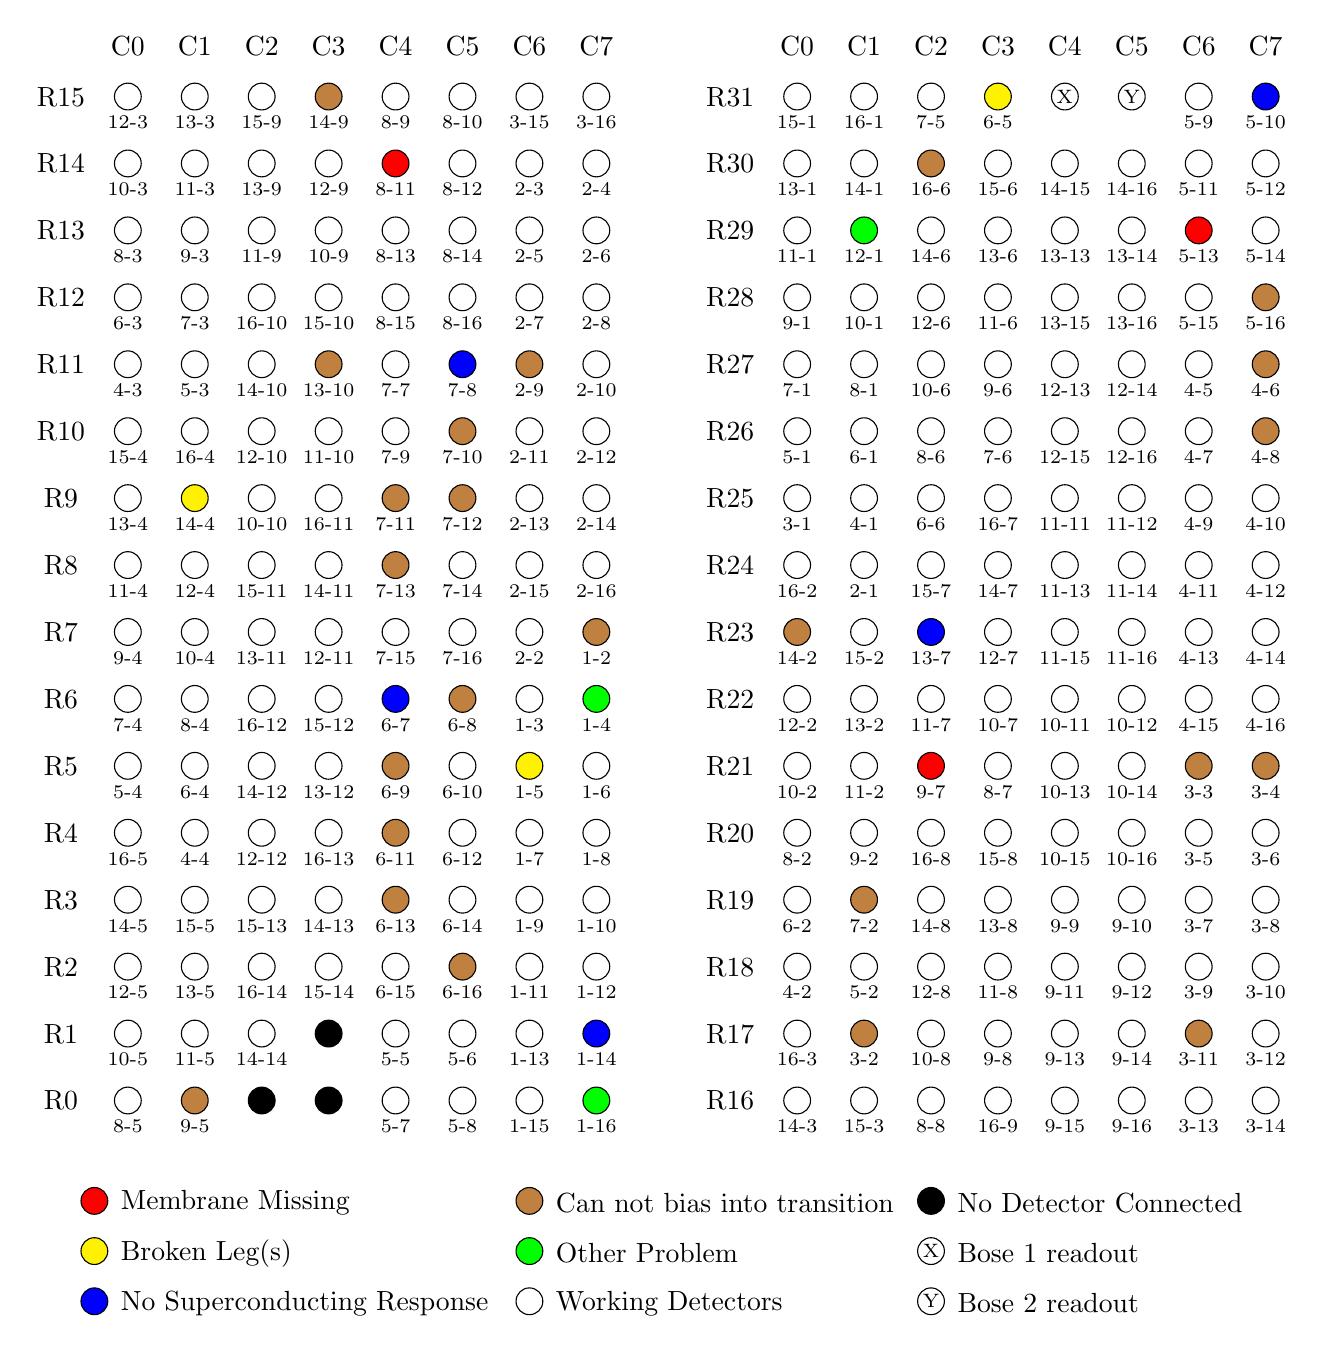
\begin{tikzpicture}[scale=0.85]
	
	%\pgfmathsetmacro{\d}{0.5}
	%\pgfmathsetmacro{\l}{2.0}
	%\pgfmathsetmacro{\D}{2}
	%\pgfmathsetmacro{\L}{2}
	%\pgfmathsetmacro{\phcy}{\l + \L - 0.5}
	%\pgfmathsetmacro{\phcy}{\l + \L - 0.5}

    \draw [fill=none] (1,1) circle [radius=0.2] +(0,-0.15) node[below,font=\scriptsize] {8-5};     \draw [fill=brown] (2,1) circle [radius=0.2] +(0,-0.15) node[below,font=\scriptsize] {9-5};     \draw [fill=none] (5,1) circle [radius=0.2] +(0,-0.15) node[below,font=\scriptsize] {5-7};     \draw [fill=none] (6,1) circle [radius=0.2] +(0,-0.15) node[below,font=\scriptsize] {5-8};     \draw [fill=none] (7,1) circle [radius=0.2] +(0,-0.15) node[below,font=\scriptsize] {1-15};     \draw [fill=green] (8,1) circle [radius=0.2] +(0,-0.15) node[below,font=\scriptsize] {1-16}; 
    \draw [fill=none] (1,2) circle [radius=0.2] +(0,-0.15) node[below,font=\scriptsize] {10-5};     \draw [fill=none] (2,2) circle [radius=0.2] +(0,-0.15) node[below,font=\scriptsize] {11-5};     \draw [fill=none] (3,2) circle [radius=0.2] +(0,-0.15) node[below,font=\scriptsize] {14-14};     \draw [fill=none] (5,2) circle [radius=0.2] +(0,-0.15) node[below,font=\scriptsize] {5-5};     \draw [fill=none] (6,2) circle [radius=0.2] +(0,-0.15) node[below,font=\scriptsize] {5-6};     \draw [fill=none] (7,2) circle [radius=0.2] +(0,-0.15) node[below,font=\scriptsize] {1-13};     \draw [fill=blue] (8,2) circle [radius=0.2] +(0,-0.15) node[below,font=\scriptsize] {1-14}; 
    \draw [fill=none] (1,3) circle [radius=0.2] +(0,-0.15) node[below,font=\scriptsize] {12-5};     \draw [fill=none] (2,3) circle [radius=0.2] +(0,-0.15) node[below,font=\scriptsize] {13-5};     \draw [fill=none] (3,3) circle [radius=0.2] +(0,-0.15) node[below,font=\scriptsize] {16-14};     \draw [fill=none] (4,3) circle [radius=0.2] +(0,-0.15) node[below,font=\scriptsize] {15-14};     \draw [fill=none] (5,3) circle [radius=0.2] +(0,-0.15) node[below,font=\scriptsize] {6-15};     \draw [fill=brown] (6,3) circle [radius=0.2] +(0,-0.15) node[below,font=\scriptsize] {6-16};     \draw [fill=none] (7,3) circle [radius=0.2] +(0,-0.15) node[below,font=\scriptsize] {1-11};     \draw [fill=none] (8,3) circle [radius=0.2] +(0,-0.15) node[below,font=\scriptsize] {1-12}; 
    \draw [fill=none] (1,4) circle [radius=0.2] +(0,-0.15) node[below,font=\scriptsize] {14-5};     \draw [fill=none] (2,4) circle [radius=0.2] +(0,-0.15) node[below,font=\scriptsize] {15-5};     \draw [fill=none] (3,4) circle [radius=0.2] +(0,-0.15) node[below,font=\scriptsize] {15-13};     \draw [fill=none] (4,4) circle [radius=0.2] +(0,-0.15) node[below,font=\scriptsize] {14-13};     \draw [fill=brown] (5,4) circle [radius=0.2] +(0,-0.15) node[below,font=\scriptsize] {6-13};     \draw [fill=none] (6,4) circle [radius=0.2] +(0,-0.15) node[below,font=\scriptsize] {6-14};     \draw [fill=none] (7,4) circle [radius=0.2] +(0,-0.15) node[below,font=\scriptsize] {1-9};     \draw [fill=none] (8,4) circle [radius=0.2] +(0,-0.15) node[below,font=\scriptsize] {1-10}; 
    \draw [fill=none] (1,5) circle [radius=0.2] +(0,-0.15) node[below,font=\scriptsize] {16-5};     \draw [fill=none] (2,5) circle [radius=0.2] +(0,-0.15) node[below,font=\scriptsize] {4-4};     \draw [fill=none] (3,5) circle [radius=0.2] +(0,-0.15) node[below,font=\scriptsize] {12-12};     \draw [fill=none] (4,5) circle [radius=0.2] +(0,-0.15) node[below,font=\scriptsize] {16-13};     \draw [fill=brown] (5,5) circle [radius=0.2] +(0,-0.15) node[below,font=\scriptsize] {6-11};     \draw [fill=none] (6,5) circle [radius=0.2] +(0,-0.15) node[below,font=\scriptsize] {6-12};     \draw [fill=none] (7,5) circle [radius=0.2] +(0,-0.15) node[below,font=\scriptsize] {1-7};     \draw [fill=none] (8,5) circle [radius=0.2] +(0,-0.15) node[below,font=\scriptsize] {1-8}; 
    \draw [fill=none] (1,6) circle [radius=0.2] +(0,-0.15) node[below,font=\scriptsize] {5-4};     \draw [fill=none] (2,6) circle [radius=0.2] +(0,-0.15) node[below,font=\scriptsize] {6-4};     \draw [fill=none] (3,6) circle [radius=0.2] +(0,-0.15) node[below,font=\scriptsize] {14-12};     \draw [fill=none] (4,6) circle [radius=0.2] +(0,-0.15) node[below,font=\scriptsize] {13-12};     \draw [fill=brown] (5,6) circle [radius=0.2] +(0,-0.15) node[below,font=\scriptsize] {6-9};     \draw [fill=none] (6,6) circle [radius=0.2] +(0,-0.15) node[below,font=\scriptsize] {6-10};     \draw [fill=yellow] (7,6) circle [radius=0.2] +(0,-0.15) node[below,font=\scriptsize] {1-5};     \draw [fill=none] (8,6) circle [radius=0.2] +(0,-0.15) node[below,font=\scriptsize] {1-6}; 
    \draw [fill=none] (1,7) circle [radius=0.2] +(0,-0.15) node[below,font=\scriptsize] {7-4};     \draw [fill=none] (2,7) circle [radius=0.2] +(0,-0.15) node[below,font=\scriptsize] {8-4};     \draw [fill=none] (3,7) circle [radius=0.2] +(0,-0.15) node[below,font=\scriptsize] {16-12};     \draw [fill=none] (4,7) circle [radius=0.2] +(0,-0.15) node[below,font=\scriptsize] {15-12};     \draw [fill=blue] (5,7) circle [radius=0.2] +(0,-0.15) node[below,font=\scriptsize] {6-7};     \draw [fill=brown] (6,7) circle [radius=0.2] +(0,-0.15) node[below,font=\scriptsize] {6-8};     \draw [fill=none] (7,7) circle [radius=0.2] +(0,-0.15) node[below,font=\scriptsize] {1-3};     \draw [fill=green] (8,7) circle [radius=0.2] +(0,-0.15) node[below,font=\scriptsize] {1-4}; 
    \draw [fill=none] (1,8) circle [radius=0.2] +(0,-0.15) node[below,font=\scriptsize] {9-4};     \draw [fill=none] (2,8) circle [radius=0.2] +(0,-0.15) node[below,font=\scriptsize] {10-4};     \draw [fill=none] (3,8) circle [radius=0.2] +(0,-0.15) node[below,font=\scriptsize] {13-11};     \draw [fill=none] (4,8) circle [radius=0.2] +(0,-0.15) node[below,font=\scriptsize] {12-11};     \draw [fill=none] (5,8) circle [radius=0.2] +(0,-0.15) node[below,font=\scriptsize] {7-15};     \draw [fill=none] (6,8) circle [radius=0.2] +(0,-0.15) node[below,font=\scriptsize] {7-16};     \draw [fill=none] (7,8) circle [radius=0.2] +(0,-0.15) node[below,font=\scriptsize] {2-2};     \draw [fill=brown] (8,8) circle [radius=0.2] +(0,-0.15) node[below,font=\scriptsize] {1-2}; 
    \draw [fill=none] (1,9) circle [radius=0.2] +(0,-0.15) node[below,font=\scriptsize] {11-4};     \draw [fill=none] (2,9) circle [radius=0.2] +(0,-0.15) node[below,font=\scriptsize] {12-4};     \draw [fill=none] (3,9) circle [radius=0.2] +(0,-0.15) node[below,font=\scriptsize] {15-11};     \draw [fill=none] (4,9) circle [radius=0.2] +(0,-0.15) node[below,font=\scriptsize] {14-11};     \draw [fill=brown] (5,9) circle [radius=0.2] +(0,-0.15) node[below,font=\scriptsize] {7-13};     \draw [fill=none] (6,9) circle [radius=0.2] +(0,-0.15) node[below,font=\scriptsize] {7-14};     \draw [fill=none] (7,9) circle [radius=0.2] +(0,-0.15) node[below,font=\scriptsize] {2-15};     \draw [fill=none] (8,9) circle [radius=0.2] +(0,-0.15) node[below,font=\scriptsize] {2-16}; 
    \draw [fill=none] (1,10) circle [radius=0.2] +(0,-0.15) node[below,font=\scriptsize] {13-4};     \draw [fill=yellow] (2,10) circle [radius=0.2] +(0,-0.15) node[below,font=\scriptsize] {14-4};     \draw [fill=none] (3,10) circle [radius=0.2] +(0,-0.15) node[below,font=\scriptsize] {10-10};     \draw [fill=none] (4,10) circle [radius=0.2] +(0,-0.15) node[below,font=\scriptsize] {16-11};     \draw [fill=brown] (5,10) circle [radius=0.2] +(0,-0.15) node[below,font=\scriptsize] {7-11};     \draw [fill=brown] (6,10) circle [radius=0.2] +(0,-0.15) node[below,font=\scriptsize] {7-12};     \draw [fill=none] (7,10) circle [radius=0.2] +(0,-0.15) node[below,font=\scriptsize] {2-13};     \draw [fill=none] (8,10) circle [radius=0.2] +(0,-0.15) node[below,font=\scriptsize] {2-14}; 
    \draw [fill=none] (1,11) circle [radius=0.2] +(0,-0.15) node[below,font=\scriptsize] {15-4};     \draw [fill=none] (2,11) circle [radius=0.2] +(0,-0.15) node[below,font=\scriptsize] {16-4};     \draw [fill=none] (3,11) circle [radius=0.2] +(0,-0.15) node[below,font=\scriptsize] {12-10};     \draw [fill=none] (4,11) circle [radius=0.2] +(0,-0.15) node[below,font=\scriptsize] {11-10};     \draw [fill=none] (5,11) circle [radius=0.2] +(0,-0.15) node[below,font=\scriptsize] {7-9};     \draw [fill=brown] (6,11) circle [radius=0.2] +(0,-0.15) node[below,font=\scriptsize] {7-10};     \draw [fill=none] (7,11) circle [radius=0.2] +(0,-0.15) node[below,font=\scriptsize] {2-11};     \draw [fill=none] (8,11) circle [radius=0.2] +(0,-0.15) node[below,font=\scriptsize] {2-12}; 
    \draw [fill=none] (1,12) circle [radius=0.2] +(0,-0.15) node[below,font=\scriptsize] {4-3};     \draw [fill=none] (2,12) circle [radius=0.2] +(0,-0.15) node[below,font=\scriptsize] {5-3};     \draw [fill=none] (3,12) circle [radius=0.2] +(0,-0.15) node[below,font=\scriptsize] {14-10};     \draw [fill=brown] (4,12) circle [radius=0.2] +(0,-0.15) node[below,font=\scriptsize] {13-10};     \draw [fill=none] (5,12) circle [radius=0.2] +(0,-0.15) node[below,font=\scriptsize] {7-7};     \draw [fill=blue] (6,12) circle [radius=0.2] +(0,-0.15) node[below,font=\scriptsize] {7-8};     \draw [fill=brown] (7,12) circle [radius=0.2] +(0,-0.15) node[below,font=\scriptsize] {2-9};     \draw [fill=none] (8,12) circle [radius=0.2] +(0,-0.15) node[below,font=\scriptsize] {2-10}; 
    \draw [fill=none] (1,13) circle [radius=0.2] +(0,-0.15) node[below,font=\scriptsize] {6-3};     \draw [fill=none] (2,13) circle [radius=0.2] +(0,-0.15) node[below,font=\scriptsize] {7-3};     \draw [fill=none] (3,13) circle [radius=0.2] +(0,-0.15) node[below,font=\scriptsize] {16-10};     \draw [fill=none] (4,13) circle [radius=0.2] +(0,-0.15) node[below,font=\scriptsize] {15-10};     \draw [fill=none] (5,13) circle [radius=0.2] +(0,-0.15) node[below,font=\scriptsize] {8-15};     \draw [fill=none] (6,13) circle [radius=0.2] +(0,-0.15) node[below,font=\scriptsize] {8-16};     \draw [fill=none] (7,13) circle [radius=0.2] +(0,-0.15) node[below,font=\scriptsize] {2-7};     \draw [fill=none] (8,13) circle [radius=0.2] +(0,-0.15) node[below,font=\scriptsize] {2-8}; 
    \draw [fill=none] (1,14) circle [radius=0.2] +(0,-0.15) node[below,font=\scriptsize] {8-3};     \draw [fill=none] (2,14) circle [radius=0.2] +(0,-0.15) node[below,font=\scriptsize] {9-3};     \draw [fill=none] (3,14) circle [radius=0.2] +(0,-0.15) node[below,font=\scriptsize] {11-9};     \draw [fill=none] (4,14) circle [radius=0.2] +(0,-0.15) node[below,font=\scriptsize] {10-9};     \draw [fill=none] (5,14) circle [radius=0.2] +(0,-0.15) node[below,font=\scriptsize] {8-13};     \draw [fill=none] (6,14) circle [radius=0.2] +(0,-0.15) node[below,font=\scriptsize] {8-14};     \draw [fill=none] (7,14) circle [radius=0.2] +(0,-0.15) node[below,font=\scriptsize] {2-5};     \draw [fill=none] (8,14) circle [radius=0.2] +(0,-0.15) node[below,font=\scriptsize] {2-6}; 
    \draw [fill=none] (1,15) circle [radius=0.2] +(0,-0.15) node[below,font=\scriptsize] {10-3};     \draw [fill=none] (2,15) circle [radius=0.2] +(0,-0.15) node[below,font=\scriptsize] {11-3};     \draw [fill=none] (3,15) circle [radius=0.2] +(0,-0.15) node[below,font=\scriptsize] {13-9};     \draw [fill=none] (4,15) circle [radius=0.2] +(0,-0.15) node[below,font=\scriptsize] {12-9};     \draw [fill=red] (5,15) circle [radius=0.2] +(0,-0.15) node[below,font=\scriptsize] {8-11};     \draw [fill=none] (6,15) circle [radius=0.2] +(0,-0.15) node[below,font=\scriptsize] {8-12};     \draw [fill=none] (7,15) circle [radius=0.2] +(0,-0.15) node[below,font=\scriptsize] {2-3};     \draw [fill=none] (8,15) circle [radius=0.2] +(0,-0.15) node[below,font=\scriptsize] {2-4}; 
    \draw [fill=none] (1,16) circle [radius=0.2] +(0,-0.15) node[below,font=\scriptsize] {12-3};     \draw [fill=none] (2,16) circle [radius=0.2] +(0,-0.15) node[below,font=\scriptsize] {13-3};     \draw [fill=none] (3,16) circle [radius=0.2] +(0,-0.15) node[below,font=\scriptsize] {15-9};     \draw [fill=brown] (4,16) circle [radius=0.2] +(0,-0.15) node[below,font=\scriptsize] {14-9};     \draw [fill=none] (5,16) circle [radius=0.2] +(0,-0.15) node[below,font=\scriptsize] {8-9};     \draw [fill=none] (6,16) circle [radius=0.2] +(0,-0.15) node[below,font=\scriptsize] {8-10};     \draw [fill=none] (7,16) circle [radius=0.2] +(0,-0.15) node[below,font=\scriptsize] {3-15};     \draw [fill=none] (8,16) circle [radius=0.2] +(0,-0.15) node[below,font=\scriptsize] {3-16}; 
    \draw [fill=none] (11,1) circle [radius=0.2] +(0,-0.15) node[below,font=\scriptsize] {14-3};     \draw [fill=none] (12,1) circle [radius=0.2] +(0,-0.15) node[below,font=\scriptsize] {15-3};     \draw [fill=none] (13,1) circle [radius=0.2] +(0,-0.15) node[below,font=\scriptsize] {8-8};     \draw [fill=none] (14,1) circle [radius=0.2] +(0,-0.15) node[below,font=\scriptsize] {16-9};     \draw [fill=none] (15,1) circle [radius=0.2] +(0,-0.15) node[below,font=\scriptsize] {9-15};     \draw [fill=none] (16,1) circle [radius=0.2] +(0,-0.15) node[below,font=\scriptsize] {9-16};     \draw [fill=none] (17,1) circle [radius=0.2] +(0,-0.15) node[below,font=\scriptsize] {3-13};     \draw [fill=none] (18,1) circle [radius=0.2] +(0,-0.15) node[below,font=\scriptsize] {3-14}; 
    \draw [fill=none] (11,2) circle [radius=0.2] +(0,-0.15) node[below,font=\scriptsize] {16-3};     \draw [fill=brown] (12,2) circle [radius=0.2] +(0,-0.15) node[below,font=\scriptsize] {3-2};     \draw [fill=none] (13,2) circle [radius=0.2] +(0,-0.15) node[below,font=\scriptsize] {10-8};     \draw [fill=none] (14,2) circle [radius=0.2] +(0,-0.15) node[below,font=\scriptsize] {9-8};     \draw [fill=none] (15,2) circle [radius=0.2] +(0,-0.15) node[below,font=\scriptsize] {9-13};     \draw [fill=none] (16,2) circle [radius=0.2] +(0,-0.15) node[below,font=\scriptsize] {9-14};     \draw [fill=brown] (17,2) circle [radius=0.2] +(0,-0.15) node[below,font=\scriptsize] {3-11};     \draw [fill=none] (18,2) circle [radius=0.2] +(0,-0.15) node[below,font=\scriptsize] {3-12}; 
    \draw [fill=none] (11,3) circle [radius=0.2] +(0,-0.15) node[below,font=\scriptsize] {4-2};     \draw [fill=none] (12,3) circle [radius=0.2] +(0,-0.15) node[below,font=\scriptsize] {5-2};     \draw [fill=none] (13,3) circle [radius=0.2] +(0,-0.15) node[below,font=\scriptsize] {12-8};     \draw [fill=none] (14,3) circle [radius=0.2] +(0,-0.15) node[below,font=\scriptsize] {11-8};     \draw [fill=none] (15,3) circle [radius=0.2] +(0,-0.15) node[below,font=\scriptsize] {9-11};     \draw [fill=none] (16,3) circle [radius=0.2] +(0,-0.15) node[below,font=\scriptsize] {9-12};     \draw [fill=none] (17,3) circle [radius=0.2] +(0,-0.15) node[below,font=\scriptsize] {3-9};     \draw [fill=none] (18,3) circle [radius=0.2] +(0,-0.15) node[below,font=\scriptsize] {3-10}; 
    \draw [fill=none] (11,4) circle [radius=0.2] +(0,-0.15) node[below,font=\scriptsize] {6-2};     \draw [fill=brown] (12,4) circle [radius=0.2] +(0,-0.15) node[below,font=\scriptsize] {7-2};     \draw [fill=none] (13,4) circle [radius=0.2] +(0,-0.15) node[below,font=\scriptsize] {14-8};     \draw [fill=none] (14,4) circle [radius=0.2] +(0,-0.15) node[below,font=\scriptsize] {13-8};     \draw [fill=none] (15,4) circle [radius=0.2] +(0,-0.15) node[below,font=\scriptsize] {9-9};     \draw [fill=none] (16,4) circle [radius=0.2] +(0,-0.15) node[below,font=\scriptsize] {9-10};     \draw [fill=none] (17,4) circle [radius=0.2] +(0,-0.15) node[below,font=\scriptsize] {3-7};     \draw [fill=none] (18,4) circle [radius=0.2] +(0,-0.15) node[below,font=\scriptsize] {3-8}; 
    \draw [fill=none] (11,5) circle [radius=0.2] +(0,-0.15) node[below,font=\scriptsize] {8-2};     \draw [fill=none] (12,5) circle [radius=0.2] +(0,-0.15) node[below,font=\scriptsize] {9-2};     \draw [fill=none] (13,5) circle [radius=0.2] +(0,-0.15) node[below,font=\scriptsize] {16-8};     \draw [fill=none] (14,5) circle [radius=0.2] +(0,-0.15) node[below,font=\scriptsize] {15-8};     \draw [fill=none] (15,5) circle [radius=0.2] +(0,-0.15) node[below,font=\scriptsize] {10-15};     \draw [fill=none] (16,5) circle [radius=0.2] +(0,-0.15) node[below,font=\scriptsize] {10-16};     \draw [fill=none] (17,5) circle [radius=0.2] +(0,-0.15) node[below,font=\scriptsize] {3-5};     \draw [fill=none] (18,5) circle [radius=0.2] +(0,-0.15) node[below,font=\scriptsize] {3-6}; 
    \draw [fill=none] (11,6) circle [radius=0.2] +(0,-0.15) node[below,font=\scriptsize] {10-2};     \draw [fill=none] (12,6) circle [radius=0.2] +(0,-0.15) node[below,font=\scriptsize] {11-2};     \draw [fill=red] (13,6) circle [radius=0.2] +(0,-0.15) node[below,font=\scriptsize] {9-7};     \draw [fill=none] (14,6) circle [radius=0.2] +(0,-0.15) node[below,font=\scriptsize] {8-7};     \draw [fill=none] (15,6) circle [radius=0.2] +(0,-0.15) node[below,font=\scriptsize] {10-13};     \draw [fill=none] (16,6) circle [radius=0.2] +(0,-0.15) node[below,font=\scriptsize] {10-14};     \draw [fill=brown] (17,6) circle [radius=0.2] +(0,-0.15) node[below,font=\scriptsize] {3-3};     \draw [fill=brown] (18,6) circle [radius=0.2] +(0,-0.15) node[below,font=\scriptsize] {3-4}; 
    \draw [fill=none] (11,7) circle [radius=0.2] +(0,-0.15) node[below,font=\scriptsize] {12-2};     \draw [fill=none] (12,7) circle [radius=0.2] +(0,-0.15) node[below,font=\scriptsize] {13-2};     \draw [fill=none] (13,7) circle [radius=0.2] +(0,-0.15) node[below,font=\scriptsize] {11-7};     \draw [fill=none] (14,7) circle [radius=0.2] +(0,-0.15) node[below,font=\scriptsize] {10-7};     \draw [fill=none] (15,7) circle [radius=0.2] +(0,-0.15) node[below,font=\scriptsize] {10-11};     \draw [fill=none] (16,7) circle [radius=0.2] +(0,-0.15) node[below,font=\scriptsize] {10-12};     \draw [fill=none] (17,7) circle [radius=0.2] +(0,-0.15) node[below,font=\scriptsize] {4-15};     \draw [fill=none] (18,7) circle [radius=0.2] +(0,-0.15) node[below,font=\scriptsize] {4-16}; 
    \draw [fill=brown] (11,8) circle [radius=0.2] +(0,-0.15) node[below,font=\scriptsize] {14-2};     \draw [fill=none] (12,8) circle [radius=0.2] +(0,-0.15) node[below,font=\scriptsize] {15-2};     \draw [fill=blue] (13,8) circle [radius=0.2] +(0,-0.15) node[below,font=\scriptsize] {13-7};     \draw [fill=none] (14,8) circle [radius=0.2] +(0,-0.15) node[below,font=\scriptsize] {12-7};     \draw [fill=none] (15,8) circle [radius=0.2] +(0,-0.15) node[below,font=\scriptsize] {11-15};     \draw [fill=none] (16,8) circle [radius=0.2] +(0,-0.15) node[below,font=\scriptsize] {11-16};     \draw [fill=none] (17,8) circle [radius=0.2] +(0,-0.15) node[below,font=\scriptsize] {4-13};     \draw [fill=none] (18,8) circle [radius=0.2] +(0,-0.15) node[below,font=\scriptsize] {4-14}; 
    \draw [fill=none] (11,9) circle [radius=0.2] +(0,-0.15) node[below,font=\scriptsize] {16-2};     \draw [fill=none] (12,9) circle [radius=0.2] +(0,-0.15) node[below,font=\scriptsize] {2-1};     \draw [fill=none] (13,9) circle [radius=0.2] +(0,-0.15) node[below,font=\scriptsize] {15-7};     \draw [fill=none] (14,9) circle [radius=0.2] +(0,-0.15) node[below,font=\scriptsize] {14-7};     \draw [fill=none] (15,9) circle [radius=0.2] +(0,-0.15) node[below,font=\scriptsize] {11-13};     \draw [fill=none] (16,9) circle [radius=0.2] +(0,-0.15) node[below,font=\scriptsize] {11-14};     \draw [fill=none] (17,9) circle [radius=0.2] +(0,-0.15) node[below,font=\scriptsize] {4-11};     \draw [fill=none] (18,9) circle [radius=0.2] +(0,-0.15) node[below,font=\scriptsize] {4-12}; 
    \draw [fill=none] (11,10) circle [radius=0.2] +(0,-0.15) node[below,font=\scriptsize] {3-1};     \draw [fill=none] (12,10) circle [radius=0.2] +(0,-0.15) node[below,font=\scriptsize] {4-1};     \draw [fill=none] (13,10) circle [radius=0.2] +(0,-0.15) node[below,font=\scriptsize] {6-6};     \draw [fill=none] (14,10) circle [radius=0.2] +(0,-0.15) node[below,font=\scriptsize] {16-7};     \draw [fill=none] (15,10) circle [radius=0.2] +(0,-0.15) node[below,font=\scriptsize] {11-11};     \draw [fill=none] (16,10) circle [radius=0.2] +(0,-0.15) node[below,font=\scriptsize] {11-12};     \draw [fill=none] (17,10) circle [radius=0.2] +(0,-0.15) node[below,font=\scriptsize] {4-9};     \draw [fill=none] (18,10) circle [radius=0.2] +(0,-0.15) node[below,font=\scriptsize] {4-10}; 
    \draw [fill=none] (11,11) circle [radius=0.2] +(0,-0.15) node[below,font=\scriptsize] {5-1};     \draw [fill=none] (12,11) circle [radius=0.2] +(0,-0.15) node[below,font=\scriptsize] {6-1};     \draw [fill=none] (13,11) circle [radius=0.2] +(0,-0.15) node[below,font=\scriptsize] {8-6};     \draw [fill=none] (14,11) circle [radius=0.2] +(0,-0.15) node[below,font=\scriptsize] {7-6};     \draw [fill=none] (15,11) circle [radius=0.2] +(0,-0.15) node[below,font=\scriptsize] {12-15};     \draw [fill=none] (16,11) circle [radius=0.2] +(0,-0.15) node[below,font=\scriptsize] {12-16};     \draw [fill=none] (17,11) circle [radius=0.2] +(0,-0.15) node[below,font=\scriptsize] {4-7};     \draw [fill=brown] (18,11) circle [radius=0.2] +(0,-0.15) node[below,font=\scriptsize] {4-8}; 
    \draw [fill=none] (11,12) circle [radius=0.2] +(0,-0.15) node[below,font=\scriptsize] {7-1};     \draw [fill=none] (12,12) circle [radius=0.2] +(0,-0.15) node[below,font=\scriptsize] {8-1};     \draw [fill=none] (13,12) circle [radius=0.2] +(0,-0.15) node[below,font=\scriptsize] {10-6};     \draw [fill=none] (14,12) circle [radius=0.2] +(0,-0.15) node[below,font=\scriptsize] {9-6};     \draw [fill=none] (15,12) circle [radius=0.2] +(0,-0.15) node[below,font=\scriptsize] {12-13};     \draw [fill=none] (16,12) circle [radius=0.2] +(0,-0.15) node[below,font=\scriptsize] {12-14};     \draw [fill=none] (17,12) circle [radius=0.2] +(0,-0.15) node[below,font=\scriptsize] {4-5};     \draw [fill=brown] (18,12) circle [radius=0.2] +(0,-0.15) node[below,font=\scriptsize] {4-6}; 
    \draw [fill=none] (11,13) circle [radius=0.2] +(0,-0.15) node[below,font=\scriptsize] {9-1};     \draw [fill=none] (12,13) circle [radius=0.2] +(0,-0.15) node[below,font=\scriptsize] {10-1};     \draw [fill=none] (13,13) circle [radius=0.2] +(0,-0.15) node[below,font=\scriptsize] {12-6};     \draw [fill=none] (14,13) circle [radius=0.2] +(0,-0.15) node[below,font=\scriptsize] {11-6};     \draw [fill=none] (15,13) circle [radius=0.2] +(0,-0.15) node[below,font=\scriptsize] {13-15};     \draw [fill=none] (16,13) circle [radius=0.2] +(0,-0.15) node[below,font=\scriptsize] {13-16};     \draw [fill=none] (17,13) circle [radius=0.2] +(0,-0.15) node[below,font=\scriptsize] {5-15};     \draw [fill=brown] (18,13) circle [radius=0.2] +(0,-0.15) node[below,font=\scriptsize] {5-16}; 
    \draw [fill=none] (11,14) circle [radius=0.2] +(0,-0.15) node[below,font=\scriptsize] {11-1};     \draw [fill=green] (12,14) circle [radius=0.2] +(0,-0.15) node[below,font=\scriptsize] {12-1};     \draw [fill=none] (13,14) circle [radius=0.2] +(0,-0.15) node[below,font=\scriptsize] {14-6};     \draw [fill=none] (14,14) circle [radius=0.2] +(0,-0.15) node[below,font=\scriptsize] {13-6};     \draw [fill=none] (15,14) circle [radius=0.2] +(0,-0.15) node[below,font=\scriptsize] {13-13};     \draw [fill=none] (16,14) circle [radius=0.2] +(0,-0.15) node[below,font=\scriptsize] {13-14};     \draw [fill=red] (17,14) circle [radius=0.2] +(0,-0.15) node[below,font=\scriptsize] {5-13};     \draw [fill=none] (18,14) circle [radius=0.2] +(0,-0.15) node[below,font=\scriptsize] {5-14}; 
    \draw [fill=none] (11,15) circle [radius=0.2] +(0,-0.15) node[below,font=\scriptsize] {13-1};     \draw [fill=none] (12,15) circle [radius=0.2] +(0,-0.15) node[below,font=\scriptsize] {14-1};     \draw [fill=brown] (13,15) circle [radius=0.2] +(0,-0.15) node[below,font=\scriptsize] {16-6};     \draw [fill=none] (14,15) circle [radius=0.2] +(0,-0.15) node[below,font=\scriptsize] {15-6};     \draw [fill=none] (15,15) circle [radius=0.2] +(0,-0.15) node[below,font=\scriptsize] {14-15};     \draw [fill=none] (16,15) circle [radius=0.2] +(0,-0.15) node[below,font=\scriptsize] {14-16};     \draw [fill=none] (17,15) circle [radius=0.2] +(0,-0.15) node[below,font=\scriptsize] {5-11};     \draw [fill=none] (18,15) circle [radius=0.2] +(0,-0.15) node[below,font=\scriptsize] {5-12}; 
    \draw [fill=none] (11,16) circle [radius=0.2] +(0,-0.15) node[below,font=\scriptsize] {15-1};     \draw [fill=none] (12,16) circle [radius=0.2] +(0,-0.15) node[below,font=\scriptsize] {16-1};     \draw [fill=none] (13,16) circle [radius=0.2] +(0,-0.15) node[below,font=\scriptsize] {7-5};     \draw [fill=yellow] (14,16) circle [radius=0.2] +(0,-0.15) node[below,font=\scriptsize] {6-5};     \draw [fill=none] (17,16) circle [radius=0.2] +(0,-0.15) node[below,font=\scriptsize] {5-9};     \draw [fill=blue] (18,16) circle [radius=0.2] +(0,-0.15) node[below,font=\scriptsize] {5-10}; 
    \draw [fill=black] (3,1) circle [radius=0.2];
    \draw [fill=black] (4,1) circle [radius=0.2];
    \draw [fill=black] (4,2) circle [radius=0.2];
    \draw [fill=none] (15,16) circle [radius=0.2] node[font=\scriptsize] {X};
    \draw [fill=none] (16,16) circle [radius=0.2] node[font=\scriptsize] {Y};

%	% detector labels
	\foreach \x in {0,...,7} \draw (1 + \x, 16.75) node {C\x};
    \foreach \x in {0,...,7} \draw (11 + \x, 16.75) node {C\x};
	\foreach \y in {0,...,15} \draw (0, 1 + \y) node {R\y};
	\foreach \y in {16,...,31} \draw (10, 1 + \y - 16) node {R\y};

	% legend
	\draw [fill=red] (0.5,-0.5) circle [radius=0.2] +(0.25,-0.03) node[right] {Membrane Missing};
	\draw [fill=yellow] (0.5,-1.25) circle [radius=0.2] +(0.25,-0.03) node[right] {Broken Leg(s)};
	\draw [fill=blue] (0.5,-2.0) circle [radius=0.2] +(0.25,-0.03) node[right] {No Superconducting Response};
	
	\draw [fill=brown] (7,-0.5) circle [radius=0.2] +(0.25,-0.03) node[right] {Can not bias into transition};
	\draw [fill=green] (7,-1.25) circle [radius=0.2] +(0.25,-0.03) node[right] {Other Problem};
	\draw [fill=none] (7,-2.0) circle [radius=0.2] +(0.25,-0.03) node[right] {Working Detectors};

	\draw [fill=black] (13,-0.5) circle [radius=0.2] +(0.25,-0.03) node[right] {No Detector Connected};
	\draw [fill=none] (13,-1.25) circle [radius=0.2] node[font=\scriptsize] {X} +(0.25,-0.03) node[right] {Bose \DISP1 readout};
	\draw [fill=none] (13,-2.0) circle [radius=0.2] node[font=\scriptsize] {Y}  +(0.25,-0.03) node[right] {Bose \DISP2 readout};




\end{tikzpicture}
\end{document}

\caption{Figure showing same information as \figref{fig:detector-cuts-wafer}, but organized in term of readout rows/columns. Each detector is labeled (below) with it's position on the detector wafer. The rows/columns are labeled on the left and top. Unused row/columns as well as the row/columns used to readout the position of the secondary mirror are also indicated. }
\label{fig:detector-cuts-rc}
\end{figure*}


\section{Readout of Mirror Position}\label{s:mirror-readout}

The \Imager\ produces a time-ordered data stream containing the output of each detector as a function of time.
In order to turn this data stream into a video, we must know where the optical system is pointing at all times.
This pointing information is placed directly into the timestream by the \Imager, as described in this section.
It is also necessary to know where each detector is pointed relative to the optical system; this relative detector pointing information is extracted from beam maps, as discussed in \sectionref{s:beam-maps}.

The pointing of the optical system is set by the positions of the two actuators --- \DISP1 and \DISP2 --- that move the secondary mirror.
The actuator control hardware provides two voltage signal which are proportional to the positions of the actuators.
This voltage signal is sent into the \Imager\ cryostat by a pair coaxial cables.
Inside the cryostat two 1-m long PhBr \AWG36 twisted pair wires carry the signal to the focal plane, where the signal is fed into the input coil of a 1st stage \SQUID.
Series resistors (4.23~M\Ohm\ for \DISP1, 4.36~M\Ohm\ for \DISP2) are used at room temperature to reduce the current flowing through the wires to a value appropriate for the 1st stage \SQUID\ input; approximately 10~\uA.

This approach allows the readout system to readout the position of the actuators in exactly the same way that it reads out the detector response.
The actuator position is synchronized perfectly with the detector data.

A natural question is whether cross-talk appears between the actuator readout and the other detectors.
To test this both actuator were moved in a 0.1~Hz sine-wave pattern over their maximum displacement range of +/- 3.5~mm, while the detectors were in the superconducting state.
Both actuators were moved at the same time, roughly 135\textdegree out of phase.
The level of crosstalk present can be quantified by performing a least-squares fit of each detector timestream $\vect{d}_{rc}$ to the model
\begin{equation}
	 \vect{d}_{rc} = A_1 \vect{d}_{\DISP1} + A_2 \vect{d}_{\DISP2}.
\end{equation}
Here $\vect{d}_{\DISP1}$ and $\vect{d}_{\DISP2}$ are the measured outputs for each actuator.
The maximum values of $|A_1|$  and $|A_2|$ are 0.0011 and 0.0014, respectively.
\figref{xxx} contains a plot summarizing these results.

An additional question is whether the actuator readout leads to higher noise.
xxx show results of this measurement.

% xxx - I get 500 uW for the load from these four wires (300 K - 1K). Can this be correct? I'm sure I did this calculation in the past and got a much smaller number. Did I screw up in the past? Is today's calculation in error? Am I intercepting this load at 50~K or 4~K, and I forgot about that? Did I use a much longer wire than 1~m? This could be a big cryogenic problem!

\section{Focus Distance}\label{s:focus-distance}

As described in \sectionref{s:optical-design}, the \Imager\ is designed to focus at distances of 16~m -- 30~m (xxx check 2nd distance).
All results described in this chapter were with the \Imager\ configured to focus at 16~m.
To check the actual distance to the target focal plane, beam maps as described in \sectionref{s:beam-maps} were performed with the blackbody source located at different distance from the cryostat.
\figref{fig:beam-vs-distance} shows beam maps for the same detector taken at different distances.
It is clear from this plot that the best focus occurs at $\sim$17~m, and the depth-of-field is approximately xxx~m.

The reasons for the difference from \ZEMAX\ predictions are not understood.
Possibilities include the cryostat being located too close to the primary mirror and the primary (or secondary) mirrors having an incorrect shape.

\section{Beam Maps}

As discussed in \sectionref{s:feedhorn-design}, the \Imager\ feedhorns are predicted to have beams that are circularly symmetric and well-approximated by Gaussians with \FWHM\ of x.xx~cm at the target.
To verify these predictions beam maps were performed by rastering the beams over a small, stationary 1030~\degC blackbody source.

The blackbody source used was an IR Labs xxx\footnote{IRLabs, Inc. Tucson, AZ. USA}.
This source reaches a maximum of 1030~\degC and has apertures ranging in size from x.xx in to x.xx in.
Best results were achieved by covering an area around the blackbody source with Aluminum foil; this eliminated hotspots in the image due to the warmth of the housing of the blackbody source itself.
\figref{xxx} shows a picture of the blackbody source with Aluminum foil mask.

The \Imager\ beams were rastered over the blackbody source by moving one actuator at xx~Hz while the other actuator moved much more slowly at xx~Hz.
This produces the path shown in \figref{xxx}.
The data stream for each detector was ``binned'' as described in \sectionref{xxx} to produce a beam map for each detector.
xxx did I remove any polynomials?
xxx need to discuss dimensional conversion factors
A 2-D Gaussian allowing for ellipticity was then fit to each beam map.
Only the points withing xxx~cm of the map peak were included in the fit.

\figref{xxx} shows the resulting beam maps.
xxx describe this plot.

xxx compare to predictions.